\documentclass[11pt, a4paper,twocolumn]{jarticle}
\usepackage[dvipdfmx]{graphicx}
\usepackage{docmute}
\begin{document}
%=============================================================
\section{Frequency filters \\based on operational amplifiers ($4^{th} \& 5^{th} day$)}
\subsubsection{Purpose}
増幅器を使いlow-pass filter, high-pass filter 作り,それを用いて周波数時間特性を調べる.
\subsection{Equipment}
\begin{itemize}
    \item 実験3と同様のもの
\end{itemize}
\subsubsection{Procedure}
まず図\ref{fig:12}に示すようにLow-pass-filterを作る.
この時オペアンプのパワーラインとGNDに前回同様0.1$\mu$Fのコンデンサを挟むことを確認する.
今回の実験ではファンクションジェネレーターを用いて矩形波,正弦波を作る.
まず$V_{in}$にファンクションジェネレーターを用いて矩形波を入力とし,10Hzから10KHzまで10倍づつ変化させながら測定した.
この時オシロスコープを用いて矩形波の入力電圧と出力電圧を同時に表示して観察した.
またこの時のデータをUSBに保存した.
次に正弦波を同様の手順で測定し記録した.

次に図\ref{fig:13}に示すようにHigh-pass-filterを作り,前回同様ファンクションジェネレーターにより矩形波の入力電圧と出力電圧の関係を測定し,次に正弦波の入力電圧と出力電圧の関係を測定した.

最後に図\ref{fig:14}に示すようにBand-pass-filterを作り,前回同様に矩形波,正弦波の入力電圧においてそれぞれ周波数を変えながら測定を行なった.

これらの実験から得られた結果を対数グラフにプロットすることによって周波数と振幅の関係について調べる.
また出力電圧の波形と入力電圧の波形を見比べてその位相差について調べる.

\begin{figure}[htbp]
 \begin{center}
  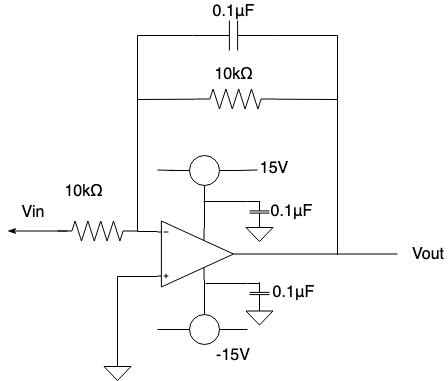
\includegraphics[width=0.8\linewidth]{fig12.png}
 \end{center}
 \caption{High pass filter}
 \label{fig:12}
\end{figure}

\begin{figure}[htbp]
 \begin{center}
  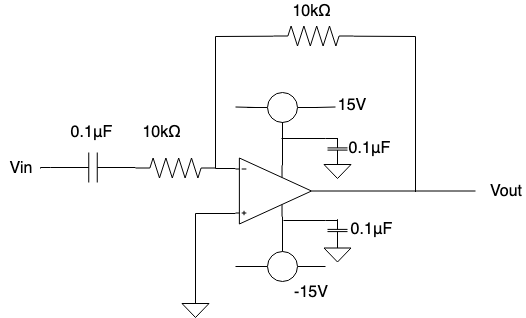
\includegraphics[width=0.8\linewidth]{fig13.png}
 \end{center}
 \caption{Low pass filter}
 \label{fig:13}
\end{figure}

\begin{figure}[htbp]
 \begin{center}
  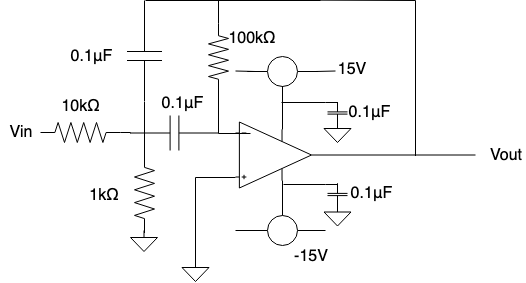
\includegraphics[width=0.8\linewidth]{fig14.png}
 \end{center}
 \caption{Band pass filter}
 \label{fig:14}
\end{figure}

\subsubsection{Result}
測定の結果まず,Low pass filterについて以下のような結果が得られた.
まずは矩形波についての結果をしめす.

\begin{figure}[htbp]
 \begin{center}
  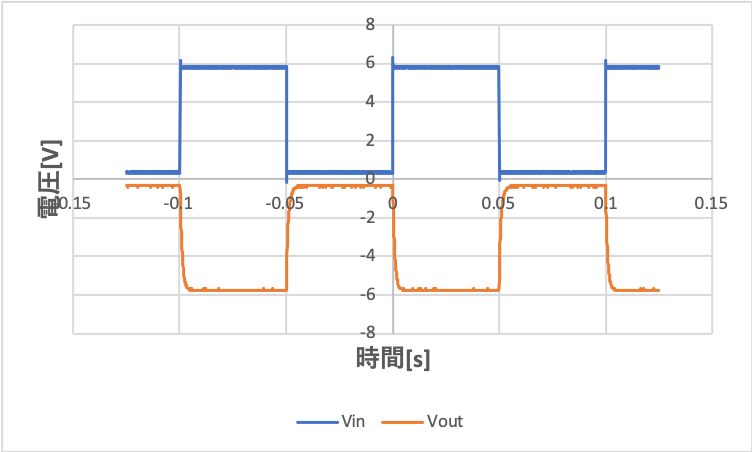
\includegraphics[width=0.8\linewidth]{fig31.png}
 \end{center}
 \caption{Low pass filter(Vin 10Hz)}
 \label{fig:31}
\end{figure}

\begin{figure}[htbp]
 \begin{center}
  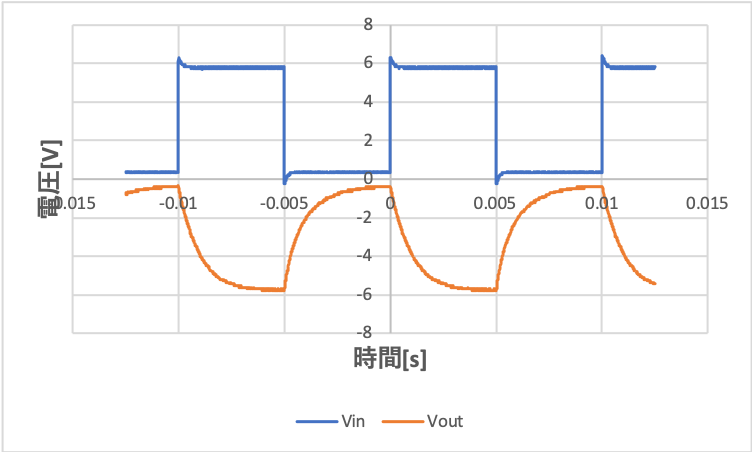
\includegraphics[width=0.8\linewidth]{fig32.png}
 \end{center}
 \caption{Low pass filter(Vin 100Hz)}
 \label{fig:32}
\end{figure}

\begin{figure}[htbp]
 \begin{center}
  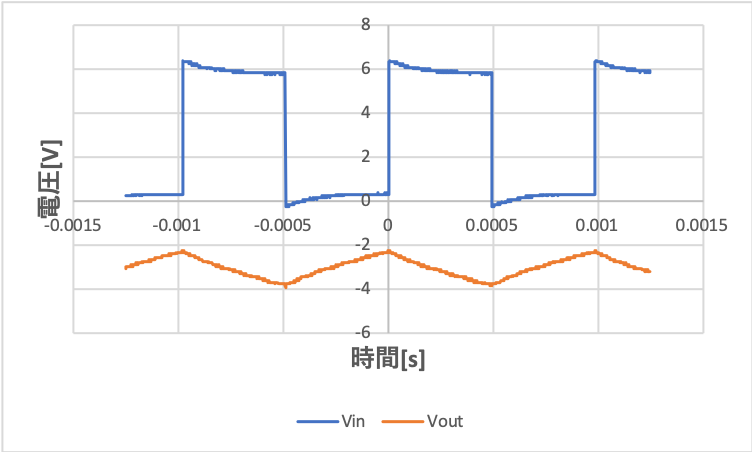
\includegraphics[width=0.8\linewidth]{fig33.png}
 \end{center}
 \caption{Low pass filter(Vin 1kHz)}
 \label{fig:33}
\end{figure}

\begin{figure}[htbp]
 \begin{center}
  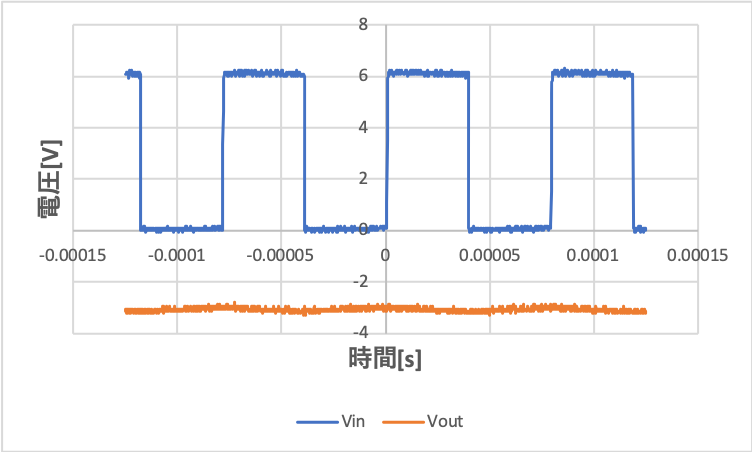
\includegraphics[width=0.8\linewidth]{fig34.png}
 \end{center}
 \caption{Low pass filter(Vin 10kHz)}
 \label{fig:34}
\end{figure}

\newpage

続いて正弦波についての結果を示す.

\begin{figure}[htbp]
 \begin{center}
  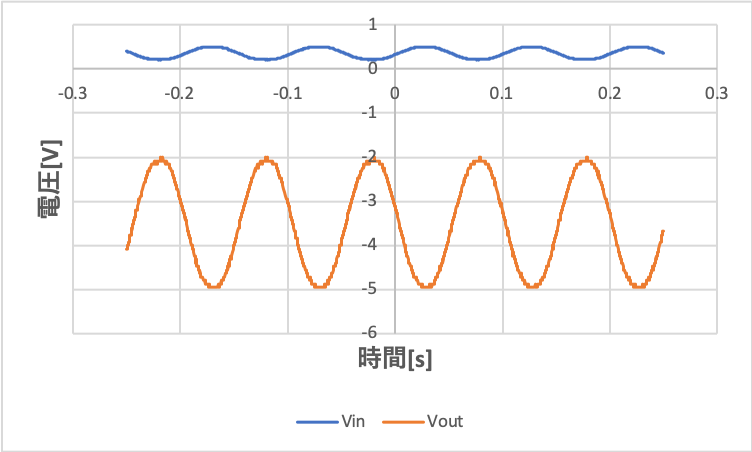
\includegraphics[width=0.8\linewidth]{fig35.png}
 \end{center}
 \caption{Low pass filter(Vin 10Hz)}
 \label{fig:35}
\end{figure}

\begin{figure}[htbp]
 \begin{center}
  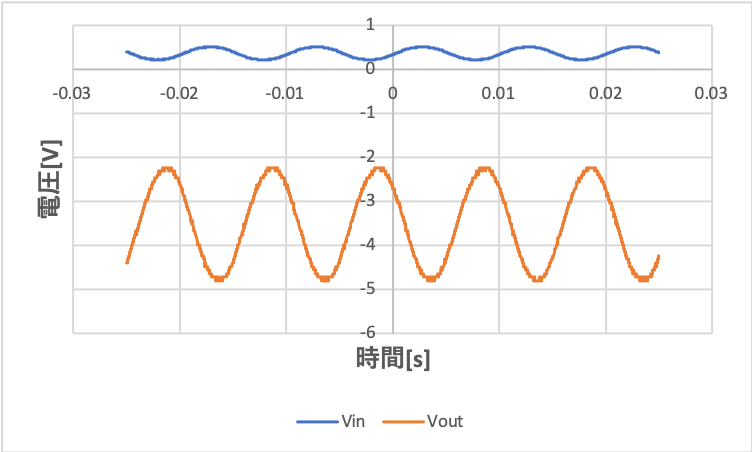
\includegraphics[width=0.8\linewidth]{fig36.png}
 \end{center}
 \caption{Low pass filter(Vin 100Hz)}
 \label{fig:36}
\end{figure}

\begin{figure}[htbp]
 \begin{center}
  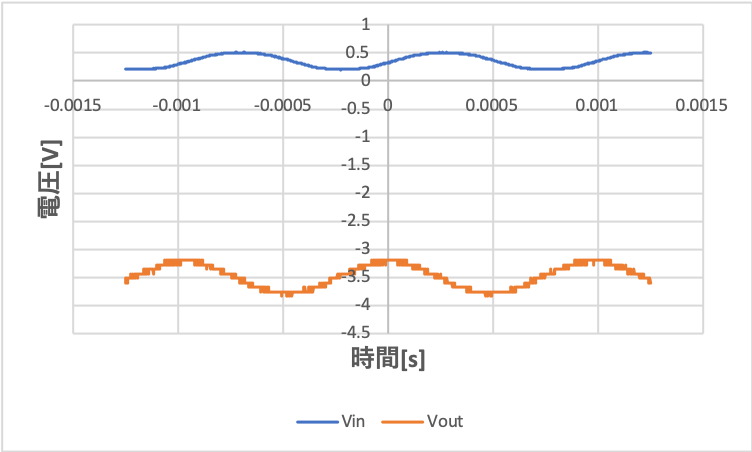
\includegraphics[width=0.8\linewidth]{fig37.png}
 \end{center}
 \caption{Low pass filter(Vin 1kHz)}
 \label{fig:37}
\end{figure}

\begin{figure}[htbp]
 \begin{center}
  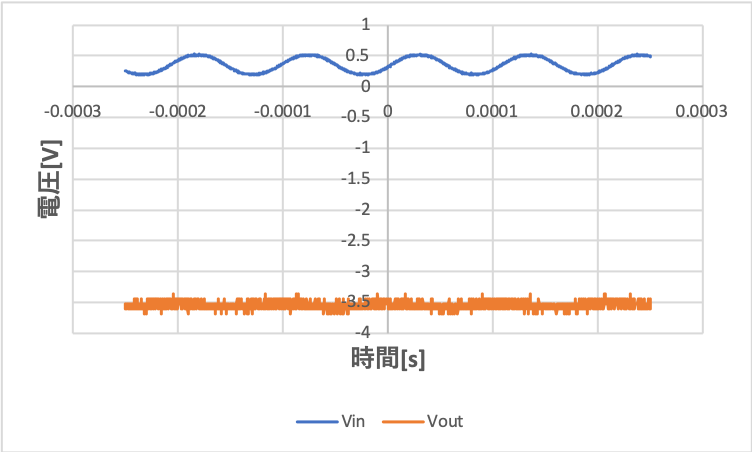
\includegraphics[width=0.8\linewidth]{fig38.png}
 \end{center}
 \caption{Low pass filter(Vin 10kHz)}
 \label{fig:38}
\end{figure}

\newpage

さらにHigh pass filterについても以下のような結果が得られた.
まずは矩形波の結果を示す.

\begin{figure}[htbp]
 \begin{center}
  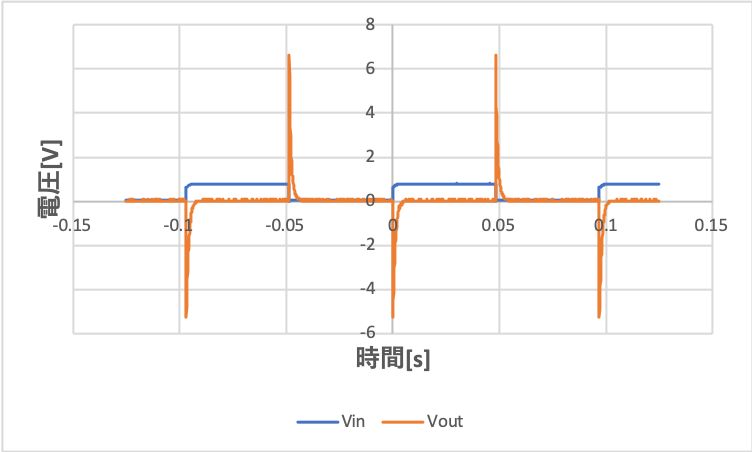
\includegraphics[width=0.8\linewidth]{fig39.png}
 \end{center}
 \caption{High pass filter(Vin 10Hz)}
 \label{fig:39}
\end{figure}

\begin{figure}[htbp]
 \begin{center}
  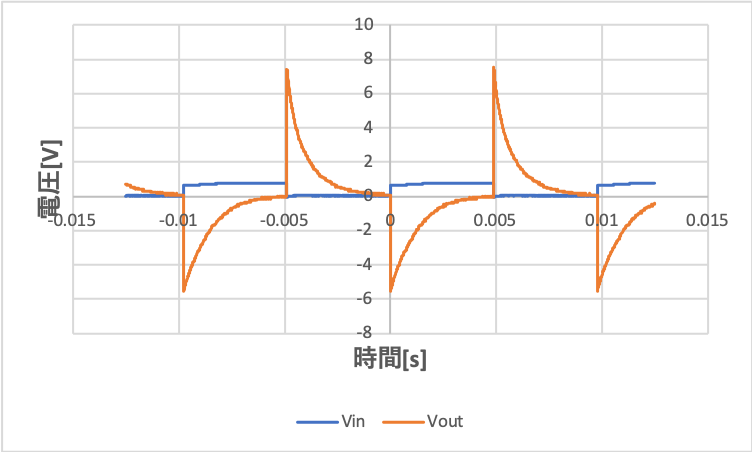
\includegraphics[width=0.8\linewidth]{fig40.png}
 \end{center}
 \caption{High pass filter(Vin 100Hz)}
 \label{fig:40}
\end{figure}

\begin{figure}[htbp]
 \begin{center}
  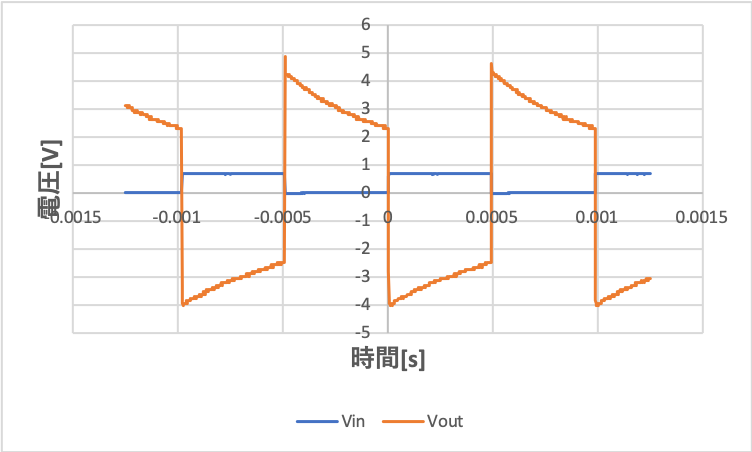
\includegraphics[width=0.8\linewidth]{fig41.png}
 \end{center}
 \caption{High pass filter(Vin 1kHz)}
 \label{fig:41}
\end{figure}

\begin{figure}[htbp]
 \begin{center}
  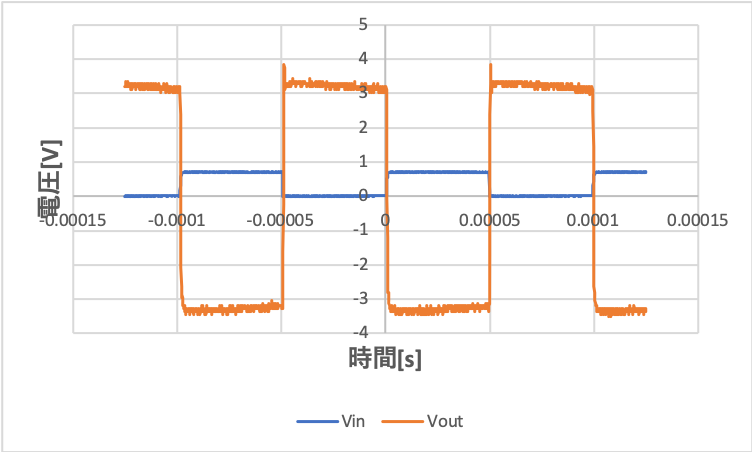
\includegraphics[width=0.8\linewidth]{fig42.png}
 \end{center}
 \caption{High pass filter(Vin 10kHz)}
 \label{fig:42}
\end{figure}

\newpage

続いて正弦波の結果を以下に示す.

\begin{figure}[htbp]
 \begin{center}
  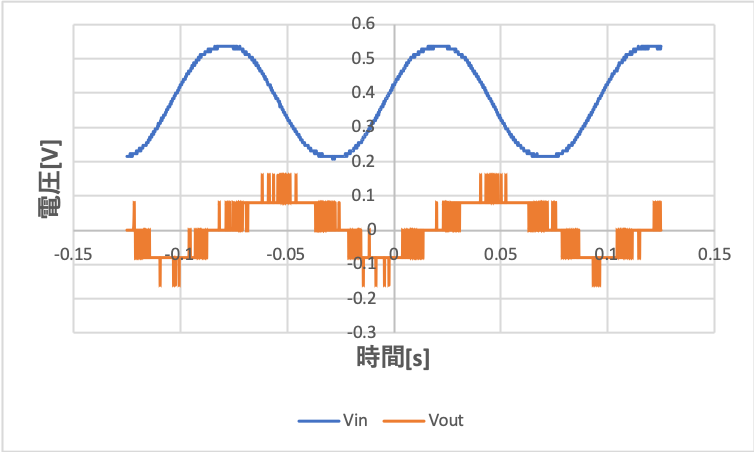
\includegraphics[width=0.8\linewidth]{fig43.png}
 \end{center}
 \caption{High pass filter(Vin 10Hz)}
 \label{fig:43}
\end{figure}

\begin{figure}[htbp]
 \begin{center}
  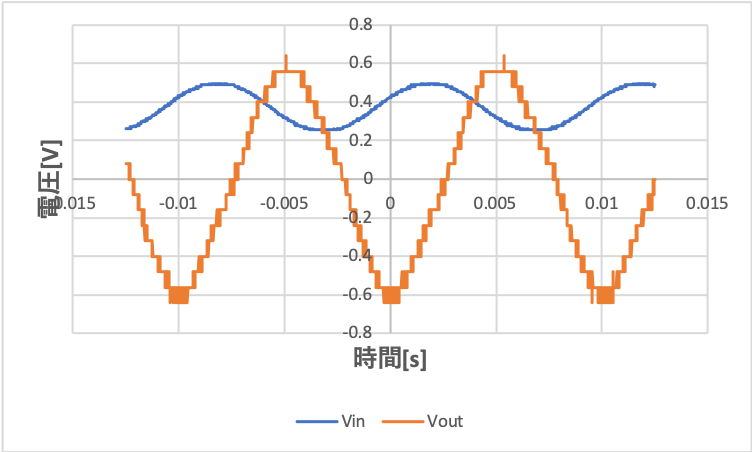
\includegraphics[width=0.8\linewidth]{fig44.png}
 \end{center}
 \caption{High pass filter(Vin 100Hz)}
 \label{fig:44}
\end{figure}

\begin{figure}[htbp]
 \begin{center}
  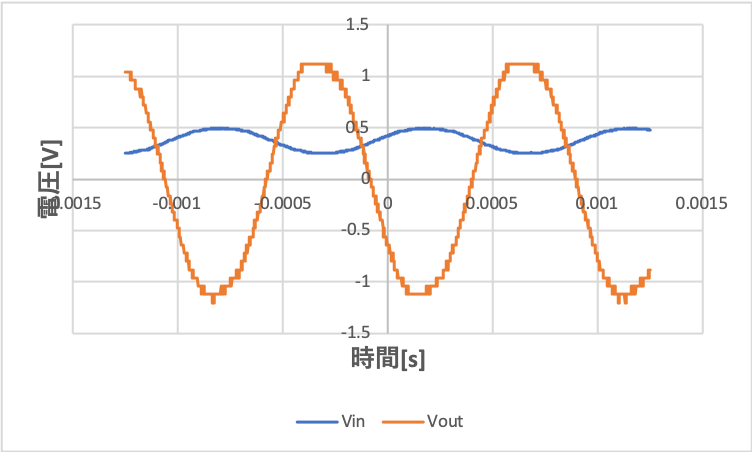
\includegraphics[width=0.8\linewidth]{fig45.png}
 \end{center}
 \caption{High pass filter(Vin 1kHz)}
 \label{fig:45}
\end{figure}

\begin{figure}[htbp]
 \begin{center}
  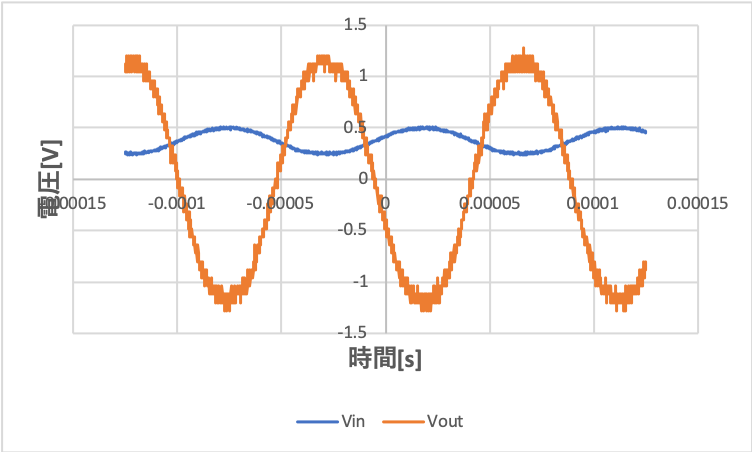
\includegraphics[width=0.8\linewidth]{fig46.png}
 \end{center}
 \caption{High pass filter(Vin 10kHz)}
 \label{fig:46}
\end{figure}

\newpage

最後にBand pass filterについても以下のような結果が得られた.
まずは矩形波の結果を示す.

\begin{figure}[htbp]
 \begin{center}
  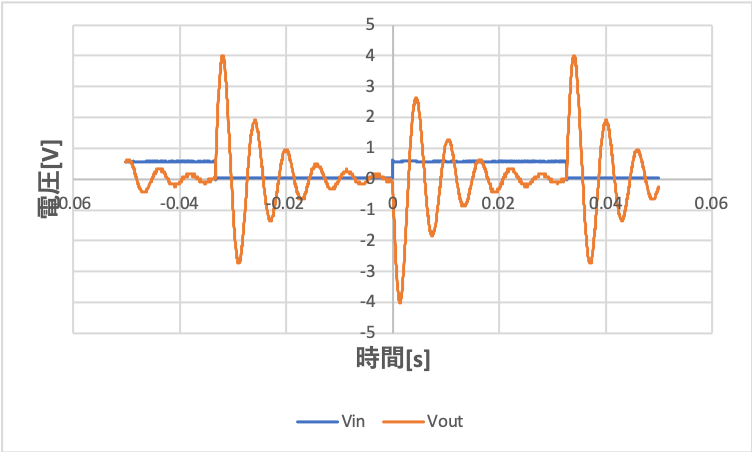
\includegraphics[width=0.8\linewidth]{fig47.png}
 \end{center}
 \caption{Band pass filter(Vin 10Hz)}
 \label{fig:47}
\end{figure}

\begin{figure}[htbp]
 \begin{center}
  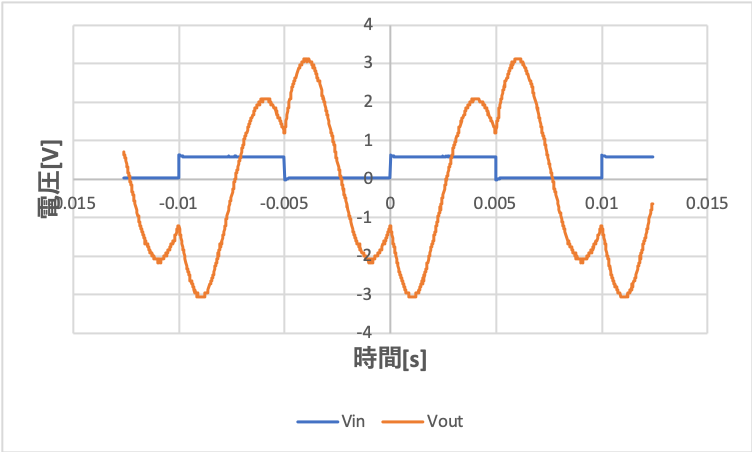
\includegraphics[width=0.8\linewidth]{fig48.png}
 \end{center}
 \caption{Band pass filter(Vin 100Hz)}
 \label{fig:48}
\end{figure}

\begin{figure}[htbp]
 \begin{center}
  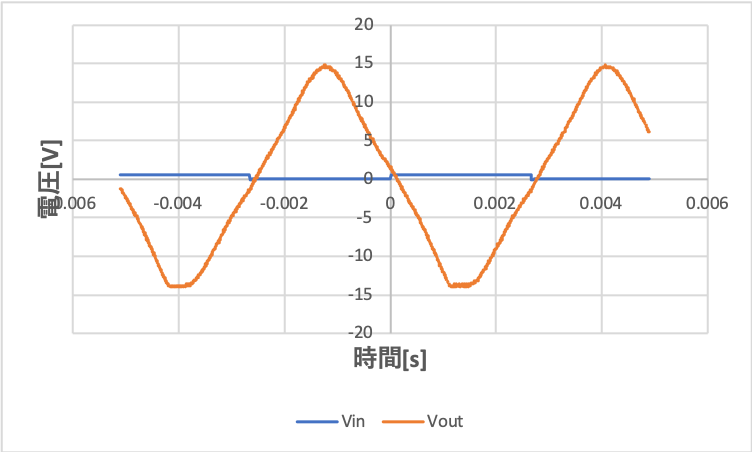
\includegraphics[width=0.8\linewidth]{fig49.png}
 \end{center}
 \caption{Band pass filter(Vin 2kHz)}
 \label{fig:49}
\end{figure}

\begin{figure}[htbp]
 \begin{center}
  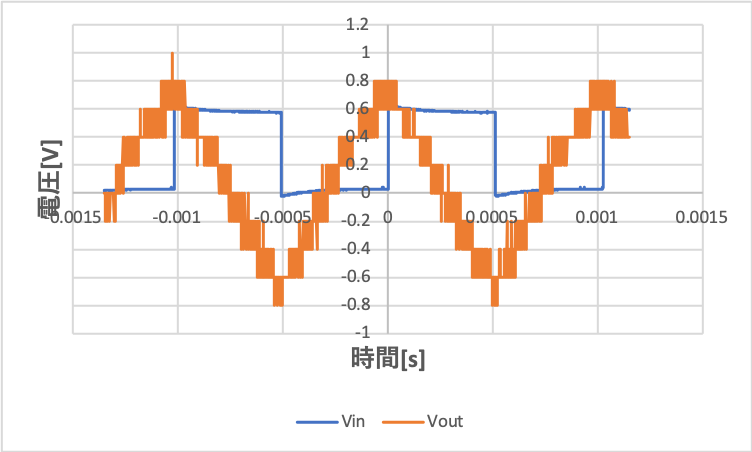
\includegraphics[width=0.8\linewidth]{fig50.png}
 \end{center}
 \caption{Band pass filter(Vin 10kHz)}
 \label{fig:50}
\end{figure}

\newpage

続いて正弦波の結果を以下に示す.

\begin{figure}[htbp]
 \begin{center}
  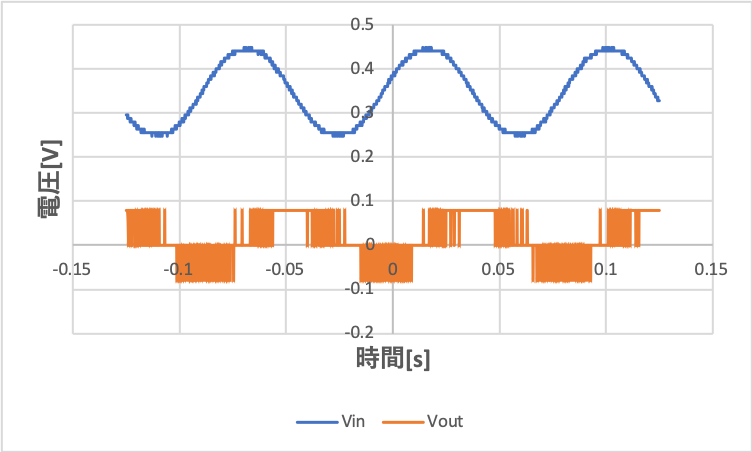
\includegraphics[width=0.8\linewidth]{fig51.png}
 \end{center}
 \caption{Band pass filter(Vin 10Hz)}
 \label{fig:51}
\end{figure}

\begin{figure}[htbp]
 \begin{center}
  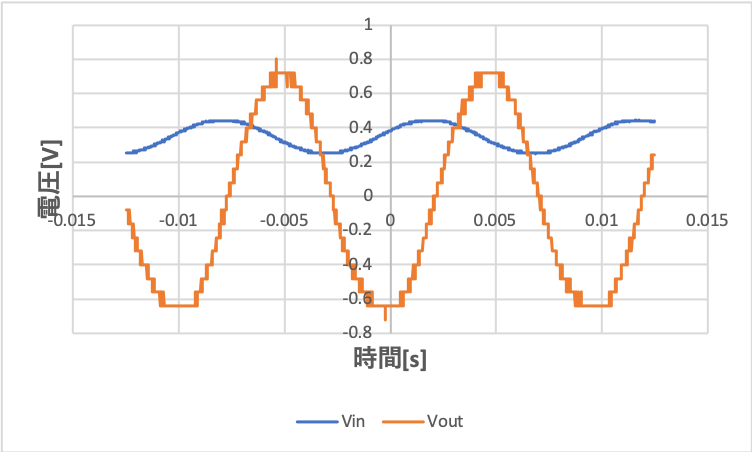
\includegraphics[width=0.8\linewidth]{fig52.png}
 \end{center}
 \caption{Band pass filter(Vin 100Hz)}
 \label{fig:52}
\end{figure}

\begin{figure}[htbp]
 \begin{center}
  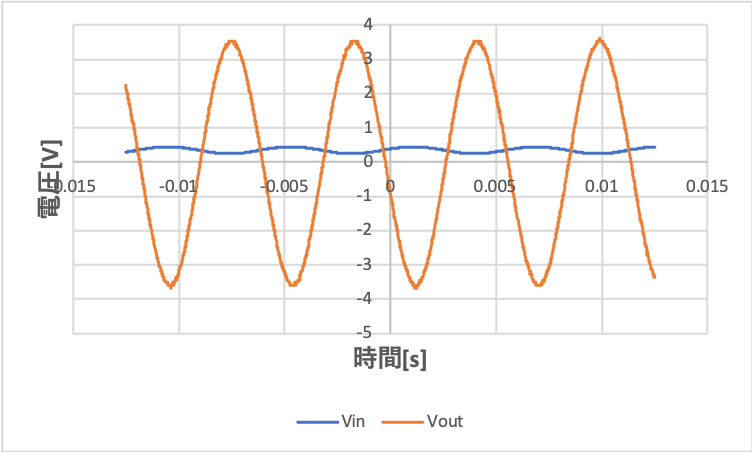
\includegraphics[width=0.8\linewidth]{fig53.png}
 \end{center}
 \caption{Band pass filter(Vin 1kHz)}
 \label{fig:53}
\end{figure}

\begin{figure}[htbp]
 \begin{center}
  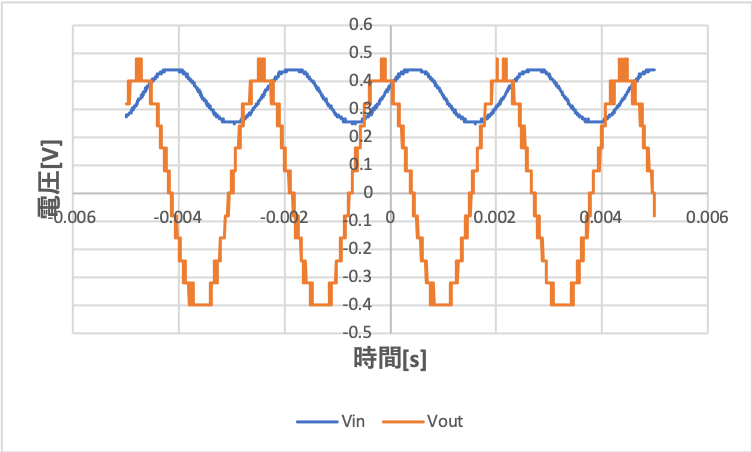
\includegraphics[width=0.8\linewidth]{fig54.png}
 \end{center}
 \caption{Band pass filter(Vin 5kHz)}
 \label{fig:54}
\end{figure}

\begin{figure}[htbp]
 \begin{center}
  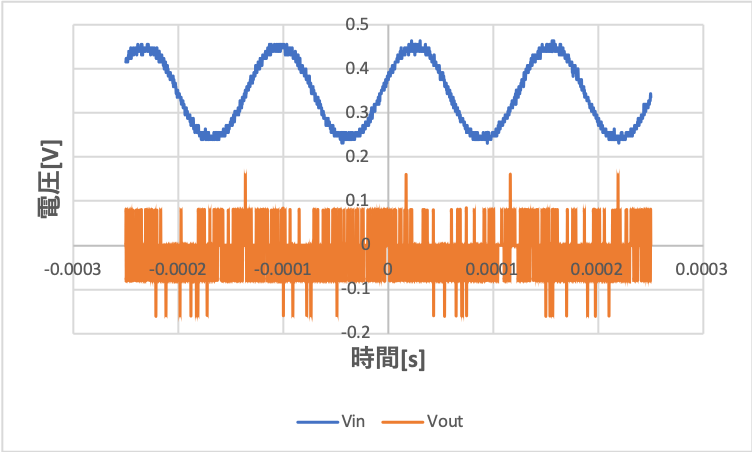
\includegraphics[width=0.8\linewidth]{fig55.png}
 \end{center}
 \caption{Band pass filter(Vin 10kHz)}
 \label{fig:55}
\end{figure}

\newpage


\documentclass[11pt, a4paper,twocolumn]{jarticle}
\usepackage[dvipdfmx]{graphicx}
\begin{document}

実験結果よりLow pass filterでは入力電圧の周波数が小さい時は元の矩形波を反転させた形の出力が得られたが,周波数が上がるにつれて元の矩形波が変化した際に遅れを生じるようになり指数関数的に追いつくような波形が得られた.
特に1kHzでの出力波は三角波のようになり,それ以上周波数が上がると出力は一定値となった.

また,High pass filterでは入力電圧の周波数が高くなるにつれて元の矩形を反転させたような出力が得られた.また低周波数領域では入力電圧が変化した瞬間だけ一瞬電圧の大きさがが大きくなりその後指数関数的に減少するような結果となった.

さらにBand pass filterでは10Hz付近では正弦波の重ね合わせのような出力が得られた.
これらの波の振幅は非常に小さかった.
また,100Hz付近になると入力の矩形波を反転させたような出力が得られた.
さらに周波数をあげると出力は一定値となった.

またそれぞれの場合において正弦波の入力を与えるとLow pass filterでは高周波数領域で振幅が小さくなり,High pass filterでは低周波数領域で振幅が小さくなり,Band pass filterでは低周波数領域と高周波数領域で振幅が小さくなった.
また総じてカットされる周波数での出力波は滑らかではなく不連続な波となった.

\subsubsection{Discussion}
今回はなぜ低周波数領域や高周波数領域の入力をカットできるのかを考察していく.
まず,図\ref{fig:13},図\ref{fig:14},図\ref{fig:15}における回路は前回の実験で行なった反転増幅回路とほぼ同じ構造をしているのがわかる.
そのことより今回の出力は入力を反転させたような波形であると予測できる.

Low pass filterについて考察を行う.
図\ref{fig:13}の回路においてキルヒホッフの法則を用いると以下の微分方程式を立てることができる.
\begin{equation}
    RC\frac{dV_{out}}{dt} + V_{out} = -V_{in}
\end{equation}

この微分方程式をとくと以下のような式を得る.
\begin{equation}
    V_{out} = -u(t)\left[1-exp\left(-\frac{t}{RC}\right)\right]
\end{equation}

この式よりtが十分大きい時expの部分は0に近づくため出力は入力の反転した値が出てくる.
一方で高周波の場合はexpは1に近づくので出力は0に近づいていくこととなり実験結果と一致することが確かめられた.

次にHigh pass filterについて考察を行う.
図\ref{fig:14}の回路においてキルヒホッフの法則を用いると以下の微分方程式を立てることができる.
\begin{equation}
    V_{out} = -RC\frac{d}{dt}(V_{out}+V_{in})
\end{equation}

この微分方程式をとくと以下のような式を得る.
\begin{equation}
    V_{out} = -u(t)exp\left(-\frac{t}{RC}\right)\
\end{equation}

この式よりtが十分小さい時expの値は1に近づくこととなり出力は入力の反転した値となる.
またtが十分大きい時はexpの値は0に近づくこととなり結果的に出力は0となる.
この性質は高周波数成分を通し,低周波数成分をカットする性質であるので実験の値とも一致することが確かめられた.

ここで得られた特定の周波数をカットするフィルターの応用例について考えてみる.
例えば,画像や音声において人間の目に見えないもしくは聞き取ることができない周波数成分はデータとして余計なのでフィルターに通してカットすることで,元のデータ量を落とすことができる.

\end{document}


%=============================================================
\newpage
\end{document}
